\appendix
\renewcommand{\thesection}{\Alph{section}}
\chapter*{Appendix}
\addcontentsline{toc}{chapter}{Appendix}


\section{Other Approaches to Clustering}\label{\positionnumber}
Other approaches to clustering include:
\begin{itemize}
    \item \textbf{Grid-based methods} construct a grid on the space to cluster that may be scaled to produce clusters in multiple resolutions. Most grid-based methods have a fast processing time as they are typically independent of the number of data objects but rather on the space the objects span.
    
    \item \textbf{Bi-clustering methods} sometimes also referred to as subspace clustering clusters the objects and one class of attributes - in other words rows and columns of a matrix - at the same time or in the terms of Formal Concept Analysis all attributes of in the same scaling context. It is closely related to formal concept analysis as described by\cite{ignatov2012concept} and may be thought of as grouping both the columns and the rows of a table concurrently. It is a very common technique in clustering gene expression data~\cite{PONTES2015163}. An example of is given in fig. \ref{fig:biclust}. \fig{img/bicluster.jpg}{biclust}{An example of biclustering on gene expression data~\cite{PONTES2015163}.}{0.5}

    \item \textbf{Evolutionary or genetic methods} are search-based, searching the space by 
        \begin{enumerate}
            \item applying random alternations (mutation) or combinations of previous clusters to generate new clustering candidates.
            \item evaluating the so generated clustering candidates against the objective function.
            \item selecting a subset of the evaluated candidates, possibly introducing randomness and other tools to sample from different regions of the search space in order not to converge into a local minimum.
            \item iterate until there is convergence or stopping criteria are satisfied.
        \end{enumerate}
        All of these steps may be adapted to a certain setting. It is a common approach to combine evolutionary algorithms with other techniques e.g.~self-organizing maps with evolutionary algorithms~\cite{leng2006design}. 
        Generally neural networks and evolutionary algorithms or similar constructed Markov decision processes (reinforcement learning) are often combined into neural architecture search systems, using stochastic processes to select and vary the already evaluated networks to generate new ones with faster convergence rates to better AUC-scores\cite{kandasamy2018neural}. \\
        Evolutionary algorithms may be seen as Markov chains, as the Markov property holds (each generation only depends on the last one) and each generative operator creates a new candidate solution with each candidate solution having a certain probability depending on the nature of the operation and the probabilities of all generateable candidate solutions of 1 per operator and generation~\cite{Nix1992}.
\end{itemize}

\section{An Introduction to Probability Theory}\label{\positionnumber}
Probability theory is essential to understand and implement probabilistic model-based approaches like COBWEB~\cite{Fisher1987} and will be used in chapters 3 to 5. \\
There are many textbooks extensively defining the notations needed in probability theory~\cite{Baron:2013:PSC:2536837, fahrmeir2016statistik}. The following is a summary of the most important terms used in the latter chapters.\\

A \textbf{sample space $\Omega$} is the set of all possible atomic results or outcomes of an experiment. An \textbf{event E} is a subset of the sample space, i.e.~a set of elementary results or outcomes. As an example the a match day of a soccer league. Each match day 2n teams compete in n matches. The sample space would be all possible results $\Omega = \{ (i,j)| \forall i,j \in \mathbf{N}\}$. An event would e.g. be the set of results of a match day or a partial result. \\

A \textbf{$\sigma$-algebra} on sample space $\Omega$ is a collection of events $\mathfrak{E} \subseteq 2^{\Omega}$ is a pair $(\Omega, \mathfrak{E})$ with
\begin{enumerate}
    \item $\Omega \in \mathfrak{E}$
    \item $E \in \Omega: E \in \mathfrak{E} \Rightarrow \Omega \setminus E \in \mathfrak{E}$
    \item $E_0, E_1, \dots \in \mathfrak{E} \Rightarrow E_0 \cup E_1 \cup \dots \in \mathfrak{E}$
\end{enumerate}
The pair $(\Omega, \mathfrak{E})$ is then called measurable space. \\

A \textbf{probability space $\mathcal{P} = (\Omega, \mathfrak{E}, P)$} is a structure with
\begin{enumerate}
    \item $(\Omega, \mathfrak{E})$ is a $\sigma$-Algebra
    \item $\forall x \in \Omega: 0 \leq P(x) \leq 1$
    \item $P(\Omega) = 1$
    \item $\forall i \geq 0 \wedge i \neq j: E_i \cap E_j = \emptyset: P(\cup_i E_i) = \sum_i P(E_i)$ 
\end{enumerate}
$P$ is called the \textbf{probability measure}.
\vspace{0.5cm}
A \textbf{discrete probability space} is a probability space $(\Omega, \mathfrak{E}, P)$ where 
\[ \exists E \subseteq \Omega: \forall e \in E: \{e\} \in \mathfrak{E} \wedge \sum_{e \in E} P(\{e\}) = 1\]
If the probability space is not discrete, it is called \textbf{continuous}. \\

A \textbf{measurable function $f:\Omega_0 \rightarrow \Omega_1$} is a function that maps a sample space of a measurable space $(\Omega_0, \mathfrak{E}_0)$ to another sample space of another measurable space $(\Omega_1, \mathfrak{E}_1)$ with:
\[ \forall E \in \mathfrak{E}: f^{-1}(E) = \{ e | f(e) \in E \} \in \mathfrak{E} \]

A \textbf{random variable $X: \Omega \rightarrow \mathbf{R}$} is a measurable function that maps a sample space to the real numbers. \\
The \textbf{Probability distribution $P_X$} of X is given by \[ P_X = P \circ X^{-1} \]

A \textbf{distribution function $F_X$}, also called probability mass function for discrete probability space or cumulative density function for continuous probability spaces of a random variable X is given by \[ x \in \mathbf{R}: F_X(x) = P(\{e \in \Omega | X(e) \leq x\}) \]
For the discrete case it can be formulated as: \[ x \in \mathbf{R}: F_X(x) = \sum_{x_i \leq x} P_x (X = x_i) \]
In the continuous case with $f$ the probability density function: \[ x \in \mathbf{R}: F_X(x) = \int^d f_X(x) dx \]



\section{Pseudo-Code for Chapter 3: Algorithms}\label{\positionnumber}
\subsection{Hierarchical Clustering}\label{\positionnumber}
\subsubsection{Hierarchical Agglomerative Clustering}\label{\positionnumber}
\begin{algorithm}[htp]
    \KwIn{A distance matrix $dM$ of shape $|O| \times |O|$}
    \Parameters{Distance function d}
    \KwOut{A linkage matrix $lM$}
    \hrulealg
    \Begin{
        List cluster $\rightarrow$ initializeObjectsAsOwnCluster(M)\;
        \While{cluster.size() > 2}{
            m1, m2 $\rightarrow \text{argmin}_{r_1, r_2 \in \text{dM}}d(r_1, r_2)$\;
            cluster $\rightarrow (cluster \setminus m1 \setminus m2) \cup (m_1 \cup m_2)$
            dM $\rightarrow$ computePairwiseDistance(cluster)\;
        }
        \Return cluster\;
    }
\caption{Hierarchical Agglomerative Clustering}\label{agglo}
\end{algorithm}
As we need to compute the pairwise (symmetric) distance matrix which is a square matrix the space complexity of this algorithm is in $\frac{1}{2} n^2 \in \mathcal{O}(n^2)$. The time complexity is $\mathcal{O}(n^3)$ for a naive implementation as in the pseudo-code above. In each iteration we need to scan the distance matrix for the minimum and update it after merging resulting in  $2 \cdot \frac{1}{2} n^2$ steps per iteration. As in each step exactly 2 objects are merged, there are $n-1$ merges in total, resulting in a time complexity of $n - 1 \cdot n^2 \in \mathcal{O}(n^3)$.


\subsubsection{Robust Single Linkage}\label{\positionnumber}
\begin{algorithm}[htp]
    \KwIn{A distance matrix $distM$ of shape $|O| \times |O|$}
    \Parameters{$k$ the number of neighbouring points, $\alpha$ the inverse density}
    \KwOut{A linkage matrix $lM$}
    \hrulealg
    \Begin{
        Stack Clustering = new Stack\;
        \For{$o_i \in O$}{
            $r_k[o_i] = inf(\{r | k \leq |B(o_i, r)| \})$\;
        }
        $r \rightarrow 0$\;
        \While{Clustering.peek().size()$ > 1$}{
            Construct $G_r = (V_r, E_r)$ with $V_r = \{x_i \in X | r_k(x_i) \leq r\}$ and $E_r = \{i \neq j: (x_i, x_j) \in X \times X | \ ||x_i - x_j|| \leq \alpha r\}$\;
            Clusterings.push(connectedComponents($G_r$))\;
            $r++$\;
        }
        \Return Clustering\;
    }
\caption{Robust Single Linkage Clustering}\label{robust}
\end{algorithm}
The space complexity is again the space needed to store the symmetric pairwise distance matrix $\frac{1}{2}n^2 \in \mathcal{O}(n^2)$. The time complexity here is a bit different: Computing the smallest radius for which the sphere around the object contains at least k points is $n \cdot (n - 1)$ as for every object, the distance to all other points needs to be compared to $r$ - in the most naive implementation against $0, 1 \dots$ until a $r$ is found that leads to $\{o_j | \ |B(o_i, r)| \geq k$. Thus the first for loop has a complexity of $n \cdot r \cdot (n-1) \in \mathcal{O}(n^2)$. The While loop constructs a graph that needs to traverse only the list of infimum $r$ values for the vertices (i.e.~$n$ elements). Regarding the edges, the distance matrix needs to be traversed i.e.~$\frac{1}{2}n^2$ elements. As $\alpha$ is user defined, the number of iterations is variable but is less than $(n-1)$ for $\alpha = 1, k = 2$ (compare with Agglomerative clustering). To conclude, for $\alpha \geq 1$ and $k \geq 2$ convergence is faster than single linkage as many points are merged in one step. For a more comprehensive discussion of the rates of convergence, see~\cite{Chaudhuri2010RatesOC}



\subsection{Partition-based Methods}\label{\positionnumber}
\subsubsection{K-Means}\label{\positionnumber}
\begin{algorithm}[htp]density based spatial clustering 
    \KwIn{A Set of data objects $O$}
    \Parameters{$k$ the number of clusters}
    \KwOut{A set of $k$ clusters}
    \hrulealg
    \Begin{
        \For{$i = 0, \dots, k-1$}{
            Centroid $c_k \leftarrow$ Chose $k$ objects at random\;
        }
        \While{Objective function did not converge}{
            \For{$o_i \in O\setminus \{c_1, \dots c_k\}$}{
                Centroid closestCentroid = $\{c_i \in \{c_1, \dots, c_k\} | \text{argmin}_{c_i \in \{c_1, \dots, c_k\}} d(o_i, c_i)\}$
                Cluster($o_i$) = Cluster(closestCentroid)\;
            }
            \For{C $\in$ Clusters}{
                Update Centroids to the means of all objects in the cluster per feature\;
            }
        }
        \Return Clusters\;
    }
\caption{k-Means Clustering}\label{kmeans}
\end{algorithm}
The space complexity is simply the number of data objects $n \cdot k \in \mathcal{O}(n)$ for small $k$ as the distance for each object to the cluster centroid must be stored instead of the full distance matrix. The time complexity is with $I$ the number of iterations, $k$ the number of clusters and $n$ the number of objects $n \cdot k \cdot I \in \mathcal{O}(n)$ for small $k$ and $I$, as in each iteration we need to find the closest centroid to the object for each object, thus $n \cdot k$.


\subsubsection{TTSAS}\label{\positionnumber}
\begin{algorithm}[htp]
    \KwIn{A Set of data objects $O$}
    \Parameters{$\Theta_1$ the maximal distance threshold, $\Theta_2$ the minimal distance threshold}
    \KwOut{A set of $k$ clusters}
    \hrulealg
    \Begin{
        \For{$o_i \in O$}{
            categorized[$o_i$] = 0\;
        }
        k = 0 \tcp*[r]{The number of clusters}
        prev = 0    \tcp*[r]{previous iteration's change}
        curr = 0    \tcp*[r]{current iteration's change}
        exist = 0   \tcp*[r]{overall change}
        \While{$\exists o_i \in O:$ categorized[$o_i$] == 0}{
            \For{i = 1 to N}{
                \uIf{categorized[$o_i$] == 0 $\wedge$ exist$ == 0 \wedge o_i$ is the first element in the new iteration of the while loop }{
                k $\leftarrow$ k + 1\;
                $C_m = \{o_i\}$\;
                categorized[$o_i$] = 1\;
                curr = curr + 1\;
                }
                \uElseIf{categorized[$o_i$] == 0}{
                    min\_dist, min\_dist\_cluster = $\{d(o_i, C_i), C_i | \text{argmin}_{C_i \in \{C_0, \dots, C_{k- 1}\}} d(o_i, C_i)\}$\;
                    \uIf{min\_dist $< \Theta_1$}{
                        min\_dist\_cluster = min\_dist\_cluster $\cup \{o_i\}$\;
                        categorized[$o_i$] = 1\;
                        curr = curr + 1\;
                    }
                    \ElseIf{min\_dist $> \Theta_2$}{
                        k $\leftarrow$ k + 1\;
                        $C_m = \{o_i\}$\;
                        categorized[$o_i$] = 1\;
                        curr = curr + 1\;
                    }
                }
                \ElseIf{categorized[$o_i$] == 1}{
                    curr = curr + 1\;
                }
            }
            exists\_change = |current\_change - previous\_change|\;
            previous\_change = current\_change\;
            current\_change = 0\;
        }
        \Return clusters\;
    }
\caption{Two-Threshold Sequential Algorithmic Scheme Clustering}\label{ttsas}
\end{algorithm}
In algorithm\ref{ttsas} the first condition guarantees that the algorithm terminates. If the current object is uncategorized and there was no change in the last iteration and the current object is the first that is inspected in this iteration of the while loop, make it a new cluster. This results in a worst-case complexity of $n \cdot 2nk$ with $|O| = n$ and $k$ the final number of clusters after algorithm execution. in this case every object's minimal distance is between the thresholds for all clusters that are created and every point ends up in an own cluster, taking two iterations per element: The first where no change happens and a second where only one point is assigned as a new cluster and no further changes happen. For each element ($n$) do 2 complete iterations ($n \cdot 2n$), where for each element the distance to all so far existing clusters is queried ($n \cdot 2nk$), resulting in a worst-case run time of $2n^2k \in \mathcal{O}(n^3)$ as in this case $k = n$. In the best case $k << n$ and only two passes~\cite{THEODORIDIS2009627} resulting in $2 \cdot n \cdot k \in \mathcal{O}(n)$ iterations. The space complexity is as in k-Means plus $n$ to store the categorized vector.

\subsection{Density-based Methods}\label{\positionnumber}
\subsubsection{DBSCAN}\label{\positionnumber}
\begin{algorithm}[htp]
    \KwIn{A Set of data objects $O$, $o_i$ the currently expanded point, cluster[] the array storing the object to cluster mapping}
    \Parameters{$\epsilon$ the radius of the neighbourhood, MinObjects the minimal number of neighbours of a core point, cluster\_id the id of the cluster to be used}
    \KwOut{A boolean indicating weather a new cluster was formed}
    \hrulealg
    \Begin{
    seeds $\leftarrow \{o_j \in O\setminus \{o_i\} | d(o_i, o_j) \leq \epsilon \}$\;
       \uIf{seeds.size < MinObjects}{
            \Return False\;
       }
       \Else{
            \For{seed in seeds}{
                cluster[seed] = cluster\_id\;
            }
            \While{seeds $\neq \emptyset$}{
                currentSeed $\leftarrow$ seeds.pop()\;
                currentSeedNeigh = $\leftarrow \{o_j \in O\setminus \{\text{currentSeed}\}| d(o_i, o_j) \leq \epsilon \}$\;
                
                \If{currentSeedNeigh.size $\geq$ MinObjects}{
                    \For{$i = 1, \dots, $ currentSeedNeigh.size}{
                        currentResult = currentSeedNeigh[i]\;
                        \If{cluster[currentResult] == -1 $\vee$ cluster[currentResult] == 0 \tcp*[r]{i.e.~currentResult is unclassified or noise}}{
                            cluster[currentResult] = cluster\_id\;
                            \If{cluster[currentResult] == -1 \tcp*[r]{unclassified}} {
                                seeds.append(currentResult)\;
                            }
                        }
                    }
                }
            }
            \Return True\;
       }
    }
\caption{Expand Cluster method}\label{expand_cluster}
\end{algorithm} 

\begin{algorithm}[htp]
    \KwIn{A Set of data objects $O$}
    \Parameters{$\epsilon$ the radius of the neighbourhood, MinObjects the minimal number of neighbours of a core point}
    \KwOut{A set of $k$ clusters}
    \hrulealg
    \Begin{
        \For{$o_i \in O$ }{
            cluster[$o_i$] $\leftarrow$ -1 \tcp*[r]{All objects are unclassified at the start}
        }
       cluster\_id = nextId(NOISE)\;
       \For{$o_i \in O$}{
            \If{cluster[$o_i$] == -1}{
                \If{expand\_cluster($O$, $o_i$, cluster, cluster\_id, $\epsilon$, MinObjects)}{
                    cluster\_id = nextInt(cluster\_id)\;
                }
            }
       }
    }
\caption{Density-based Spatial Clustering of Applications with Noise}\label{dbscan}
\end{algorithm}
The space complexity of DBSCAN is $\frac{1}{2}n^2$ as the pairwise distance matrix needs to be computed for neighbourhood queries. The run time complexity is $n$ for the outer loop in the DBSCAN algorithm and $\log(n)$ for a neighbourhood query if the neighbourhood information is stored in an efficient data structure e.g. a R*-tree according to the authors~\cite{dbscan}. In total this induces a run time complexity of $n \log(n) \in \mathcal{O}(n \log(n))$. If no such structure is used, a neighbourhood query needs to scan a row (or column) of the matrix which takes $n$ elements to visit, resulting in $n \cdot n \in \mathcal{O}(n^2)$~\cite{han2011data}. \\


\subsubsection{OPTICS}\label{\positionnumber}
\begin{algorithm}[htp]
    \KwIn{A Set of data objects $O$, $o_i$ the currently expanded point}
    \Parameters{$\epsilon$ the radius of the neighbourhood, MinObjects the minimal number of neighbours of a core point, OrderedFile the file to write the cluster ordering to}
    \KwOut{None}
    \hrulealg
    \Begin{
    seeds $\leftarrow \{o_j \in O\setminus \{o_i\} | d(o_i, o_j) \leq \epsilon \}$\;
    $o_i$.processed $\leftarrow$ 1\;
    $o_i$.reachability\_distance = UNDEFINED\;
    $o_i$.setCoreDistance(seeds, $\epsilon$, MinObjects)\;
    OrderedFile.write($o_i$)\;
       \If{$o_i$.core\_distance $\neq$ UNDEFINED}{
       OrderSeeds.update(seeds, $o_i$)\;
            \While{OrderSeed $\neq \emptyset$}{
                currentSeed $\leftarrow$ seeds.next()\;
                seeds = $\leftarrow \{o_j \in O\setminus \{\text{currentSeed}\}| d(o_i, o_j) \leq \epsilon \}$\;
                currentSeed.preprocessed = 1\;
                currentSeed.setCoreDistance(seeds, $\epsilon$, MinObjects)\;
                OrderedFile.write(currentSeed)\;

                \If{currentSeed.core\_distance $\neq$ UNDEFINED}{
                    OrderSeeds.update(seeds, currentSeed)\;
                }
            }
       }
    }
\caption{Expand Cluster Order method}\label{expand_cluster_order}
\end{algorithm}

\begin{algorithm}[htp]
    \KwIn{neighbours a set of neighbour objects, $o_i$ the current center object}
    \Parameters{None}
    \KwOut{None}
    \hrulealg
    \Begin{
        c\_dist = $o_i$.core\_distance\;
        \For{$o_j \in$ neighbours}{
            \If{$o_j$.processed == 0}{
                new\_r\_dist = max(c\_dist, $o_i$.dist($o_j$))\;
                \uIf{ $o_j$.reachability\_distance == UNDEFINED}{
                    $o_j$.reachability\_distance = new\_r\_dist\;
                    insert($o_j$, new\_r\_dist)\;
                    }
                \Else{
                    \If{ new\_r\_dist $< o_j$.reachability\_distance}{
                        $o_j$.reachability\_distance = new\_r\_dist\;
                        decrease($o_j$, new\_r\_dist)\;
                    }
                }
            }
        }
    }
\caption{OrderSeeds.update method}\label{order_seeds_update}
\end{algorithm}

\begin{algorithm}[htp]
    \KwIn{A Set of data objects $O$}
    \Parameters{$\epsilon$ the radius of the neighbourhood, MinObjects the minimal number of neighbours of a core point, OrderedFile a file to write to}
    \KwOut{An Ordering of the clusters in the database with different densities} 
    \hrulealg
    \Begin{
        OrderedFile.open()\;
        \For{$o_i \in O$ }{
            $o_i$.processed $\leftarrow$ 0\;
        }
        \For{$o_i \in O$}{
            \If{processed[$o_i$] == 0}{
                expand\_cluster\_order($O$, $o_i$, $\epsilon$, MinObjects, OrderedFile)\;
            }
       }
       OrderedFile.close()\;
    }
\caption{Ordering Points To Identify Cluster Structure}\label{optics}
\end{algorithm}
As the algorithm proceeds very similar to DBSCAN a lot of the complexity analysis also applies here: The space complexity is $\frac{1}{2}n^2$ for the pairwise distance matrix plus additionally the file that is written to, which size depends on the number of clusters but is generally bound by $3n$ (the object plus two distances per object) what yields $\frac{1}{2}n^2 + 3n \in \mathcal{O}(n^2)$. Regarding the computational complexity, the authors provide $\mathcal{O}(n^2)$ as run time without a special data structure and $\mathcal{O}(n \log(n))$ with a specialised data structure\cite{optics}. The additional overhead for finding the appropriate core distance may be solved with a one time pass over the respective row or column using dynamic programming, i.e.~besides querying the neighbour hood to find the seeding neighbours another pass is needed to find the core distance. \\


\subsubsection{HDBSCAN}\label{\positionnumber}
\begin{algorithm}[htp]
    \KwIn{A Set of data objects $O$}
    \Parameters{MinObjects the minimal number of neighbours of a core point}
    \KwOut{A dendrogram}
    \hrulealg
    \Begin{
        \For{$o_i \in O$ }{
            compute the core distance wrt. MinObjects\;
        }
        Build the mutual reachability graph $G_{\text{MinObjects}}$\;
        Build the minimum spanning tree of $G_{\text{MinObjects}}$\;
        Add a self-edge for each vertex $v_{o_i}$ in the minimal spanning tree with weight $d_{\text{core}}(o_i)$\;
        
        Assign all objects the same label \tcp*[r]{this forms the root of the dendrogram}
        \While{$G_{\text{MinObjects}}$ has edges}{
            Set the dendrogram scale value of the current level in the hierarchy to the largest edge weight which is to be removed\;
            Remove the largest edge(s)\;
            Assign a label to the connected component, that contained the end vertices of the removed edge(s)\;
            If the end vertices are not in a connected component assign the noise label to those\;
        }
    }
\caption{Hierarchical Density-based Spatial Clustering of Applications with Noise}\label{hdbscan}
\end{algorithm}
The space requirements are the same as for DBSCAN: The pairwise distance matrix needs $\frac{1}{2}n^2 \in \mathcal{O}n^2$ space complexity. regarding the run time, one needs to compute the core-distance for each object which takes $n \cdot n \in \mathcal{O}(n^2)$. Constructing the minimum spanning tree using Prim's algorithm or Boruvka's algorithm is in $\mathcal{O}(n^2)$ worst-case run time complexity. Removing all edges iteratively requires maximally $\frac{1}{2}n^2$ iterations for a fully connected graph and when sorting the matrix before starting the removal procedure which takes $\mathcal{O}(n \log n)$ steps retrieving the maximum is a constant time operation. Overall we get $n^2 + n^2 + n \log n +\frac{1}{2}n^2 \in \mathcal{O}(n^2)$ steps as run time complexity.

\subsection{Conceptual Clustering}\label{\positionnumber}
\subsubsection{Cobweb}\label{\positionnumber}
With $b$ the average branching factor, $n$ the number of objects classified so far, $A$ the number of all distinct attributes, $V$ the average number of distinct values per attribute for categorical values. When incorporating a new object, at each level the node counts must be updated, the category utility must be computed for each child to find the host, split merge and creation must be probed. That is when computing the category utility takes $\mathcal{O}(bAV)$ steps, finding the host is $b \cdot bav$, adding the probes for merging (finding another host and computing the category utility for the operation means b+1 computations of the category utility, splitting and class creation is one time computing the category utility resulting in $(b + b + 1 + 1 + 1) \cdot bAV = (2b + 3) \cdot bAV = 2b^2AV + 3bAV \in \mathcal{O}(b^2AV)$. As the depth of the tree is $\log_B(n)$ and we need to incorporate every instance we get $n \cdot \log_b(n) \cdot \mathcal{O}(b^2AV) \in \mathcal{O}(n \cdot \log (n) \cdot b^2 AV)$. In the most naive implementation each data object needs to be stored as a leaf and additional $\frac{n}{b}$ nodes are needed to build the tree, resulting in a space complexity of $n + \frac{n}{b} \in \mathcal{O}(n)$.
\begin{algorithm}[htp]
    \KwIn{An object $o_i \in O$}
    \Parameters{node the node currently visiting}
    \KwOut{A hierarchy of clusters with concept descriptions}
    \hrulealg
    \Begin{
        updateCounts(node, $o_i$)\;
        \uIf{node is a leaf}{
            node.add\_child($o_i$)\;
        }
        \Else{
            host, host\_cu = find the child of node, that best hosts $o_i$\;
            new\_class\_cu = probeCreateNewClass($o_i$)\;
            merge\_cu = probeMerge(host, $o_i$)\;
            split\_cu = probeSplit(host)\;
            max\_cu = $\max(\text{new\_class\_cu}, \text{merge\_cu}, \text{split\_cu}, \text{host\_cu})$\;
            \uIf{max\_cu $==$ new\_class\_cu}{
                createNewClass($o_i$)\;
            }
            \uElseIf{max\_cu $==$ merge\_cu}{
                merged\_node = merge(host, $o_i$)\;
                COBWEB($o_i$, merged\_node)\;
            }
            \uElseIf{max\_cu == split\_cu}{
                split(host)\;
                COBWEB($o_i$, node)\;
            }
            \Else{
            COBWEB($o_i$, host)
            }
        }
    }
\caption{COBWEB}\label{cobweb_}
\end{algorithm}
\clearpage

\section{Example Taxonomy Extraction from a Dendrogram}\label{\positionnumber}
\begin{minipage}{0.48\textwidth}
$C_{14} = C_0 \cup C_2$, with distance 1 \\
$C_{15} = C_1 \cup C_{14}$, with distance 1 \\
$C_{16} = C_3 \cup C_{15}$, with distance 1 \\
$C_{17} = C_5 \cup C_7$, with distance 1 \\
$C_{18} = C_6 \cup C_{17}$, with distance 1 \\
$C_{19} = C_4 \cup C_{18}$, with distance 1 \\
$C_{20} = C_8 \cup C_{19}$, with distance 1 \\
$C_{21} = C_9 \cup C_{11}$, with distance 1 \\
$C_{22} = C_{12} \cup C_{21}$, with distance 1 \\
$C_{23} = C_{13} \cup C_{22}$, with distance 1 \\
$C_{24} = C_{16} \cup C_{20}$, with distance 2 \\
$C_{25} = C_{23} \cup C_{24}$, with distance 2 \\
$C_{26} = C_{10} \cup C_{25}$, with distance 2 \\
\end{minipage} \hfill
\begin{minipage}{0.48\textwidth}
\begin{minted}{text}
[
    [ 0.,  2.,  1.]
    [ 1., 14.,  1.]
    [ 3., 15.,  1.]
    [ 5.,  7.,  1.]
    [ 6., 17.,  1.]
    [ 4., 18.,  1.]
    [ 8., 19.,  1.]
    [ 9., 11.,  1.]
    [12., 21.,  1.]
    [13., 22.,  1.]
    [16., 20.,  2.]
    [23., 24.,  2.]
    [10., 25.,  2.]
 ]
 \end{minted}
\end{minipage} \\
is transformed to \\ \vspace{0.5cm}
\begin{minipage}{0.48\textwidth}
$C_{16} = C_0 \cup C_2 \cup C_1 \cup C_3$, with distance 1 \\  
$C_{20} = C_5 \cup C_7 \cup C_6 \cup C_4 \cup C_8$, with distance 1 \\ 
$C_{23} = C_9 \cup C_{11} \cup C_{12} \cup C_{13}$, with distance 1 \\ 
$C_{26} = C_{16} \cup C_{20} \cup C_{23} \cup C_{19}$, with distance 2 \\   
\end{minipage} 
\hfill
\begin{minipage}{0.48\textwidth}
\begin{minted}{text}
[
    [[ 0.,  2.,  1.,  3.], 1]
    [[ 5.,  7.,  6.,  4.,  8.], 1]
    [[ 9., 11.,  12.,  13. ], 1]
    [[16.,  20.,  23.,  10.], 2]       
 ]
 \end{minted}
\end{minipage}  
\begin{figure}[htp]
    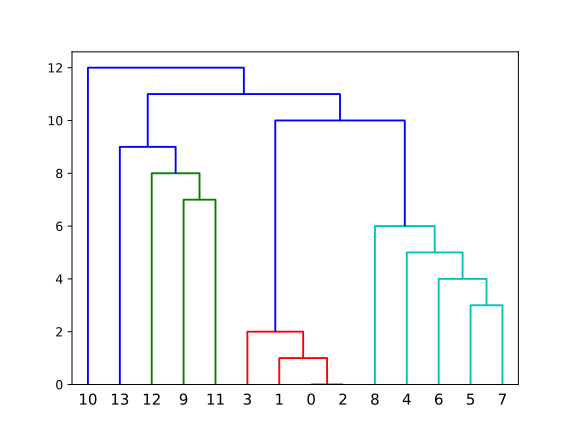
\includegraphics[width=0.49\textwidth]{img/extract_ex_dendro.png}
        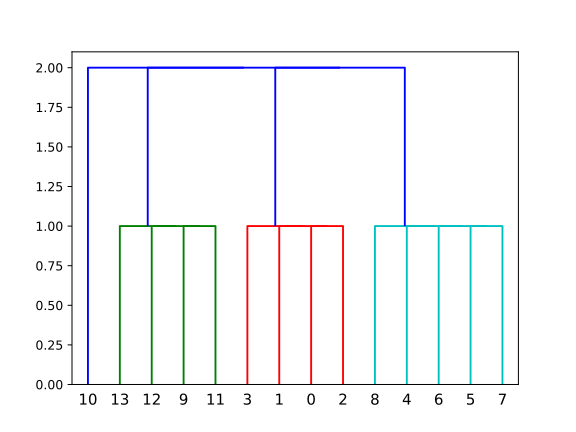
\includegraphics[width=0.49\textwidth]{img/extract_ex_taxo.png}
    \caption{The Input and output of the taxonomy extraction heuristic}
\end{figure} 
\clearpage

\section{Example Concept Descriptions}
\subsection{Labels only}

  \begin{table}[h]    \centering 
   \begin{longtable}{c c l l l} \toprule   
Attribute & ValueType & Value & Probability & Occurrences \\ \midrule \endhead \bottomrule \endfoot \endlastfoot
\multirow{1}{*}{birthday} & Numeric &  mean= 19829638.000, std=21997.377 & $0.0045$ & $9$ \\ \hline \noalign{\penalty-5000}  
\multirow{9}{*}{lastName} & Nominal & Dayan & $0.0005$ & $1$ \\* 
 & Nominal & Chen & $0.0005$ & $1$ \\* 
 & Nominal & Reddy & $0.0005$ & $1$ \\* 
 & Nominal & Gomez & $0.0005$ & $1$ \\* 
 & Nominal & Johnson & $0.0005$ & $1$ \\* 
 & Nominal & Mettacara & $0.0005$ & $1$ \\* 
 & Nominal & Takahashi & $0.0005$ & $1$ \\* 
 & Nominal & Kobayashi & $0.0005$ & $1$ \\* 
 & Nominal & Loan & $0.0005$ & $1$ \\ \hline \noalign{\penalty-5000}  
\multirow{2}{*}{gender} & Nominal & female & $0.0035$ & $7$ \\* 
 & Nominal & male & $0.0010$ & $2$ \\ \hline \noalign{\penalty-5000}  
\multirow{5}{*}{browserUsed} & Nominal & Chrome & $0.2590$ & $518$ \\* 
 & Nominal & Firefox & $0.4010$ & $802$ \\* 
 & Nominal & Internet Explorer & $0.2315$ & $463$ \\* 
 & Nominal & Safari & $0.0395$ & $79$ \\* 
 & Nominal & Opera & $0.0340$ & $68$ \\ \hline \noalign{\penalty-5000}  
\multirow{1}{*}{length} & Numeric &  mean= 29.296, std=45.025 & $0.9605$ & $1921$ \\ \hline \noalign{\penalty-5000}  
\multirow{10}{*}{Labels} & Nominal & Message & $0.9605$ & $1921$ \\* 
 & Nominal & Comment & $0.6350$ & $1270$ \\* 
 & Nominal & Forum & $0.0260$ & $52$ \\* 
 & Nominal & Post & $0.3255$ & $651$ \\* 
 & Nominal & Tag & $0.0035$ & $7$ \\* 
 & Nominal & Person & $0.0045$ & $9$ \\* 
 & Nominal & Organisation & $0.0050$ & $10$ \\* 
 & Nominal & University & $0.0040$ & $8$ \\* 
 & Nominal & Company & $0.0010$ & $2$ \\* 
 & Nominal & TagClass & $0.0005$ & $1$ \\ \hline \noalign{\penalty-5000}  
\multirow{3}{*}{language} & Nominal & tk & $0.0300$ & $60$ \\* 
 & Nominal & uz & $0.0265$ & $53$ \\* 
 & Nominal & ar & $0.0045$ & $9$ \\ \hline \noalign{\penalty-5000}  
\multirow{1}{*}{creationDate} & Numeric &  Value too large to display & $0.9910$ & $1982$ \\ \hline \noalign{\penalty-5000}  
title & Nominal & Too many values to display & & \\ \hline \noalign{\penalty-5000} 
content & Nominal & Too many values to display & & \\ \hline \noalign{\penalty-5000} 
url & Nominal & Too many values to display & & \\ \hline \noalign{\penalty-5000} 
\multirow{9}{*}{firstName} & Nominal & Ahmed & $0.0005$ & $1$ \\* 
 & Nominal & Hao & $0.0005$ & $1$ \\* 
 & Nominal & Arun & $0.0005$ & $1$ \\* 
 & Nominal & Raul & $0.0005$ & $1$ \\* 
 & Nominal & Bill & $0.0005$ & $1$ \\* 
 & Nominal & Ashin & $0.0005$ & $1$ \\* 
 & Nominal & Koji & $0.0005$ & $1$ \\* 
 & Nominal & Takeshi & $0.0005$ & $1$ \\* 
 & Nominal & Batong & $0.0005$ & $1$ \\ \hline \noalign{\penalty-5000}  
imageFile & Nominal & Too many values to display & & \\ \hline \noalign{\penalty-5000} 
name & Nominal & Too many values to display & & \\ \hline \noalign{\penalty-5000} 
locationIP & Nominal & Too many values to display & & \\ \hline \noalign{\penalty-5000} 
id & Nominal & Too many values to display & & \\ \hline \noalign{\penalty-5000} 
\caption{LDBC SNB Labels \& Node Properties: ConceptNode l, P(node) = 1.0, Count 2000}
\end{longtable}
 \end{table} 


  \begin{table}[h]    \centering 
   \begin{longtable}{c c l l l} \toprule   
Attribute & ValueType & Value & Probability & Occurrences \\ \midrule \endhead \bottomrule \endfoot \endlastfoot
\multirow{5}{*}{browserUsed} & Nominal & Firefox & $0.4003$ & $508$ \\* 
 & Nominal & Chrome & $0.2671$ & $339$ \\* 
 & Nominal & Internet Explorer & $0.2553$ & $324$ \\* 
 & Nominal & Safari & $0.0457$ & $58$ \\* 
 & Nominal & Opera & $0.0315$ & $40$ \\ \hline \noalign{\penalty-5000}  
\multirow{1}{*}{length} & Numeric &  mean= 33.433, std=43.357 & $1.0000$ & $1269$ \\ \hline \noalign{\penalty-5000}  
\multirow{3}{*}{Labels} & Nominal & Message & $1.0000$ & $1269$ \\* 
 & Nominal & Comment & $0.9976$ & $1266$ \\* 
 & Nominal & Post & $0.0024$ & $3$ \\ \hline \noalign{\penalty-5000}  
locationIP & Nominal & Too many values to display & & \\ \hline \noalign{\penalty-5000} 
\multirow{2}{*}{language} & Nominal & tk & $0.0008$ & $1$ \\* 
 & Nominal & uz & $0.0016$ & $2$ \\ \hline \noalign{\penalty-5000}  
id & Nominal & Too many values to display & & \\ \hline \noalign{\penalty-5000} 
\multirow{1}{*}{creationDate} & Numeric &  Value too large to display & $1.0000$ & $1269$ \\ \hline \noalign{\penalty-5000}  
content & Nominal & Too many values to display & & \\ \hline \noalign{\penalty-5000} 
\caption{LDBC SNB Labels \& Node Properties: ConceptNode l0, P(node) = 0.6345, Count 1269}
\end{longtable}
 \end{table} 


  \begin{table}[h]    \centering 
   \begin{longtable}{c c l l l} \toprule   
Attribute & ValueType & Value & Probability & Occurrences \\ \midrule \endhead \bottomrule \endfoot \endlastfoot
\multirow{2}{*}{browserUsed} & Nominal & Firefox & $0.9980$ & $508$ \\* 
 & Nominal & Chrome & $0.0020$ & $1$ \\ \hline \noalign{\penalty-5000}  
\multirow{1}{*}{length} & Numeric &  mean= 33.450, std=44.419 & $1.0000$ & $509$ \\ \hline \noalign{\penalty-5000}  
\multirow{3}{*}{Labels} & Nominal & Message & $1.0000$ & $509$ \\* 
 & Nominal & Comment & $0.9941$ & $506$ \\* 
 & Nominal & Post & $0.0059$ & $3$ \\ \hline \noalign{\penalty-5000}  
locationIP & Nominal & Too many values to display & & \\ \hline \noalign{\penalty-5000} 
\multirow{2}{*}{language} & Nominal & tk & $0.0020$ & $1$ \\* 
 & Nominal & uz & $0.0039$ & $2$ \\ \hline \noalign{\penalty-5000}  
id & Nominal & Too many values to display & & \\ \hline \noalign{\penalty-5000} 
\multirow{1}{*}{creationDate} & Numeric &  Value too large to display & $1.0000$ & $509$ \\ \hline \noalign{\penalty-5000}  
content & Nominal & Too many values to display & & \\ \hline \noalign{\penalty-5000} 
\caption{LDBC SNB Labels \& Node Properties: ConceptNode l00, P(node) = 0.40110323089046496, Count 509}
\end{longtable}
 \end{table} 


  \begin{table}[h]    \centering 
   \begin{longtable}{c c l l l} \toprule   
Attribute & ValueType & Value & Probability & Occurrences \\ \midrule \endhead \bottomrule \endfoot \endlastfoot
\multirow{1}{*}{browserUsed} & Nominal & Chrome & $1.0000$ & $338$ \\ \hline \noalign{\penalty-5000}  
\multirow{1}{*}{length} & Numeric &  mean= 34.814, std=43.628 & $1.0000$ & $338$ \\ \hline \noalign{\penalty-5000}  
\multirow{2}{*}{Labels} & Nominal & Message & $1.0000$ & $338$ \\* 
 & Nominal & Comment & $1.0000$ & $338$ \\ \hline \noalign{\penalty-5000}  
locationIP & Nominal & Too many values to display & & \\ \hline \noalign{\penalty-5000} 
id & Nominal & Too many values to display & & \\ \hline \noalign{\penalty-5000} 
\multirow{1}{*}{creationDate} & Numeric &  Value too large to display & $1.0000$ & $338$ \\ \hline \noalign{\penalty-5000}  
content & Nominal & Too many values to display & & \\ \hline \noalign{\penalty-5000} 
\caption{LDBC SNB Labels \& Node Properties: ConceptNode l01, P(node) = 0.26635145784081954, Count 338}
\end{longtable}
 \end{table} 


  \begin{table}[h]    \centering 
   \begin{longtable}{c c l l l} \toprule   
Attribute & ValueType & Value & Probability & Occurrences \\ \midrule \endhead \bottomrule \endfoot \endlastfoot
\multirow{3}{*}{browserUsed} & Nominal & Safari & $0.1374$ & $58$ \\* 
 & Nominal & Opera & $0.0948$ & $40$ \\* 
 & Nominal & Internet Explorer & $0.7678$ & $324$ \\ \hline \noalign{\penalty-5000}  
\multirow{1}{*}{length} & Numeric &  mean= 32.306, std=41.782 & $1.0000$ & $422$ \\ \hline \noalign{\penalty-5000}  
\multirow{2}{*}{Labels} & Nominal & Message & $1.0000$ & $422$ \\* 
 & Nominal & Comment & $1.0000$ & $422$ \\ \hline \noalign{\penalty-5000}  
locationIP & Nominal & Too many values to display & & \\ \hline \noalign{\penalty-5000} 
id & Nominal & Too many values to display & & \\ \hline \noalign{\penalty-5000} 
\multirow{1}{*}{creationDate} & Numeric &  Value too large to display & $1.0000$ & $422$ \\ \hline \noalign{\penalty-5000}  
content & Nominal & Too many values to display & & \\ \hline \noalign{\penalty-5000} 
\caption{LDBC SNB Labels \& Node Properties: ConceptNode l02, P(node) = 0.3325453112687155, Count 422}
\end{longtable}
 \end{table} 


  \begin{table}[h]    \centering 
   \begin{longtable}{c c l l l} \toprule   
Attribute & ValueType & Value & Probability & Occurrences \\ \midrule \endhead \bottomrule \endfoot \endlastfoot
\multirow{1}{*}{birthday} & Numeric &  mean= 19829638.000, std=21997.270 & $0.0123$ & $9$ \\ \hline \noalign{\penalty-5000}  
\multirow{9}{*}{lastName} & Nominal & Dayan & $0.0014$ & $1$ \\* 
 & Nominal & Reddy & $0.0014$ & $1$ \\* 
 & Nominal & Johnson & $0.0014$ & $1$ \\* 
 & Nominal & Chen & $0.0014$ & $1$ \\* 
 & Nominal & Gomez & $0.0014$ & $1$ \\* 
 & Nominal & Mettacara & $0.0014$ & $1$ \\* 
 & Nominal & Takahashi & $0.0014$ & $1$ \\* 
 & Nominal & Kobayashi & $0.0014$ & $1$ \\* 
 & Nominal & Loan & $0.0014$ & $1$ \\ \hline \noalign{\penalty-5000}  
\multirow{2}{*}{gender} & Nominal & female & $0.0096$ & $7$ \\* 
 & Nominal & male & $0.0027$ & $2$ \\ \hline \noalign{\penalty-5000}  
\multirow{5}{*}{browserUsed} & Nominal & Internet Explorer & $0.1902$ & $139$ \\* 
 & Nominal & Safari & $0.0287$ & $21$ \\* 
 & Nominal & Chrome & $0.2449$ & $179$ \\* 
 & Nominal & Opera & $0.0383$ & $28$ \\* 
 & Nominal & Firefox & $0.4022$ & $294$ \\ \hline \noalign{\penalty-5000}  
\multirow{1}{*}{length} & Numeric &  mean= 21.245, std=47.073 & $0.8919$ & $652$ \\ \hline \noalign{\penalty-5000}  
\multirow{10}{*}{Labels} & Nominal & Message & $0.8919$ & $652$ \\* 
 & Nominal & Post & $0.8865$ & $648$ \\* 
 & Nominal & Comment & $0.0055$ & $4$ \\* 
 & Nominal & Forum & $0.0711$ & $52$ \\* 
 & Nominal & Person & $0.0123$ & $9$ \\* 
 & Nominal & Tag & $0.0096$ & $7$ \\* 
 & Nominal & Organisation & $0.0137$ & $10$ \\* 
 & Nominal & University & $0.0109$ & $8$ \\* 
 & Nominal & Company & $0.0027$ & $2$ \\* 
 & Nominal & TagClass & $0.0014$ & $1$ \\ \hline \noalign{\penalty-5000}  
\multirow{3}{*}{language} & Nominal & tk & $0.0807$ & $59$ \\* 
 & Nominal & ar & $0.0123$ & $9$ \\* 
 & Nominal & uz & $0.0698$ & $51$ \\ \hline \noalign{\penalty-5000}  
\multirow{1}{*}{creationDate} & Numeric &  Value too large to display & $0.9754$ & $713$ \\ \hline \noalign{\penalty-5000}  
title & Nominal & Too many values to display & & \\ \hline \noalign{\penalty-5000} 
content & Nominal & Too many values to display & & \\ \hline \noalign{\penalty-5000} 
url & Nominal & Too many values to display & & \\ \hline \noalign{\penalty-5000} 
\multirow{9}{*}{firstName} & Nominal & Ahmed & $0.0014$ & $1$ \\* 
 & Nominal & Arun & $0.0014$ & $1$ \\* 
 & Nominal & Bill & $0.0014$ & $1$ \\* 
 & Nominal & Hao & $0.0014$ & $1$ \\* 
 & Nominal & Raul & $0.0014$ & $1$ \\* 
 & Nominal & Ashin & $0.0014$ & $1$ \\* 
 & Nominal & Koji & $0.0014$ & $1$ \\* 
 & Nominal & Takeshi & $0.0014$ & $1$ \\* 
 & Nominal & Batong & $0.0014$ & $1$ \\ \hline \noalign{\penalty-5000}  
imageFile & Nominal & Too many values to display & & \\ \hline \noalign{\penalty-5000} 
name & Nominal & Too many values to display & & \\ \hline \noalign{\penalty-5000} 
locationIP & Nominal & Too many values to display & & \\ \hline \noalign{\penalty-5000} 
id & Nominal & Too many values to display & & \\ \hline \noalign{\penalty-5000} 
\caption{LDBC SNB Labels \& Node Properties: ConceptNode l1, P(node) = 0.3655, Count 731}
\end{longtable}
 \end{table} 



  \begin{table}[h]    \centering 
   \begin{longtable}{c c l l l} \toprule   
Attribute & ValueType & Value & Probability & Occurrences \\ \midrule \endhead \bottomrule \endfoot \endlastfoot
imageFile & Nominal & Too many values to display & & \\ \hline \noalign{\penalty-5000} 
\multirow{5}{*}{browserUsed} & Nominal & Internet Explorer & $0.1959$ & $104$ \\* 
 & Nominal & Safari & $0.0358$ & $19$ \\* 
 & Nominal & Chrome & $0.2768$ & $147$ \\* 
 & Nominal & Opera & $0.0414$ & $22$ \\* 
 & Nominal & Firefox & $0.4501$ & $239$ \\ \hline \noalign{\penalty-5000}  
\multirow{1}{*}{length} & Numeric &  mean= 0.013, std=0.217 & $1.0000$ & $531$ \\ \hline \noalign{\penalty-5000}  
\multirow{3}{*}{Labels} & Nominal & Message & $1.0000$ & $531$ \\* 
 & Nominal & Post & $0.9962$ & $529$ \\* 
 & Nominal & Comment & $0.0038$ & $2$ \\ \hline \noalign{\penalty-5000}  
locationIP & Nominal & Too many values to display & & \\ \hline \noalign{\penalty-5000} 
id & Nominal & Too many values to display & & \\ \hline \noalign{\penalty-5000} 
\multirow{1}{*}{creationDate} & Numeric &  Value too large to display & $1.0000$ & $531$ \\ \hline \noalign{\penalty-5000}  
\multirow{2}{*}{content} & Nominal & fine & $0.0019$ & $1$ \\* 
 & Nominal & yes & $0.0019$ & $1$ \\ \hline \noalign{\penalty-5000}  
\caption{LDBC SNB Labels \& Node Properties: ConceptNode l10, P(node) = 0.7264021887824897, Count 531}
\end{longtable}
 \end{table} 
 

  \begin{table}[h]    \centering 
   \begin{longtable}{c c l l l} \toprule   
Attribute & ValueType & Value & Probability & Occurrences \\ \midrule \endhead \bottomrule \endfoot \endlastfoot
\multirow{1}{*}{birthday} & Numeric &  mean= 19829638.000, std=21997.270 & $0.0450$ & $9$ \\ \hline \noalign{\penalty-5000}  
\multirow{9}{*}{lastName} & Nominal & Dayan & $0.0050$ & $1$ \\* 
 & Nominal & Reddy & $0.0050$ & $1$ \\* 
 & Nominal & Johnson & $0.0050$ & $1$ \\* 
 & Nominal & Chen & $0.0050$ & $1$ \\* 
 & Nominal & Gomez & $0.0050$ & $1$ \\* 
 & Nominal & Mettacara & $0.0050$ & $1$ \\* 
 & Nominal & Takahashi & $0.0050$ & $1$ \\* 
 & Nominal & Kobayashi & $0.0050$ & $1$ \\* 
 & Nominal & Loan & $0.0050$ & $1$ \\ \hline \noalign{\penalty-5000}  
\multirow{2}{*}{gender} & Nominal & female & $0.0350$ & $7$ \\* 
 & Nominal & male & $0.0100$ & $2$ \\ \hline \noalign{\penalty-5000}  
\multirow{5}{*}{browserUsed} & Nominal & Firefox & $0.2750$ & $55$ \\* 
 & Nominal & Internet Explorer & $0.1750$ & $35$ \\* 
 & Nominal & Chrome & $0.1600$ & $32$ \\* 
 & Nominal & Opera & $0.0300$ & $6$ \\* 
 & Nominal & Safari & $0.0100$ & $2$ \\ \hline \noalign{\penalty-5000}  
\multirow{1}{*}{length} & Numeric &  mean= 114.422, std=35.776 & $0.6050$ & $121$ \\ \hline \noalign{\penalty-5000}  
\multirow{10}{*}{Labels} & Nominal & Message & $0.6050$ & $121$ \\* 
 & Nominal & Post & $0.5950$ & $119$ \\* 
 & Nominal & Forum & $0.2600$ & $52$ \\* 
 & Nominal & Person & $0.0450$ & $9$ \\* 
 & Nominal & Tag & $0.0350$ & $7$ \\* 
 & Nominal & Organisation & $0.0500$ & $10$ \\* 
 & Nominal & University & $0.0400$ & $8$ \\* 
 & Nominal & Company & $0.0100$ & $2$ \\* 
 & Nominal & TagClass & $0.0050$ & $1$ \\* 
 & Nominal & Comment & $0.0100$ & $2$ \\ \hline \noalign{\penalty-5000}  
\multirow{3}{*}{language} & Nominal & tk & $0.2950$ & $59$ \\* 
 & Nominal & ar & $0.0450$ & $9$ \\* 
 & Nominal & uz & $0.2550$ & $51$ \\ \hline \noalign{\penalty-5000}  
\multirow{1}{*}{creationDate} & Numeric &  Value too large to display & $0.9100$ & $182$ \\ \hline \noalign{\penalty-5000}  
title & Nominal & Too many values to display & & \\ \hline \noalign{\penalty-5000} 
content & Nominal & Too many values to display & & \\ \hline \noalign{\penalty-5000} 
url & Nominal & Too many values to display & & \\ \hline \noalign{\penalty-5000} 
\multirow{9}{*}{firstName} & Nominal & Ahmed & $0.0050$ & $1$ \\* 
 & Nominal & Arun & $0.0050$ & $1$ \\* 
 & Nominal & Bill & $0.0050$ & $1$ \\* 
 & Nominal & Hao & $0.0050$ & $1$ \\* 
 & Nominal & Raul & $0.0050$ & $1$ \\* 
 & Nominal & Ashin & $0.0050$ & $1$ \\* 
 & Nominal & Koji & $0.0050$ & $1$ \\* 
 & Nominal & Takeshi & $0.0050$ & $1$ \\* 
 & Nominal & Batong & $0.0050$ & $1$ \\ \hline \noalign{\penalty-5000}  
name & Nominal & Too many values to display & & \\ \hline \noalign{\penalty-5000} 
locationIP & Nominal & Too many values to display & & \\ \hline \noalign{\penalty-5000} 
id & Nominal & Too many values to display & & \\ \hline \noalign{\penalty-5000} 
\caption{LDBC SNB Labels \& Node Properties: ConceptNode l11, P(node) = 0.27359781121751026, Count 200}
\end{longtable}
 \end{table} 



\subsection{Labels, Structural Features and Characteristic Set}

  \begin{table}[h]    \centering 
   \begin{longtable}{c c l l l} \toprule   
Attribute & ValueType & Value & Probability & Occurrences \\ \midrule \endhead \bottomrule \endfoot \endlastfoot
\multirow{1}{*}{birthday} & Numeric &  mean= 19829638.000, std=21997.377 & $0.0045$ & $9$ \\ \hline \noalign{\penalty-5000}  
\multirow{9}{*}{lastName} & Nominal & Dayan & $0.0005$ & $1$ \\* 
 & Nominal & Chen & $0.0005$ & $1$ \\* 
 & Nominal & Reddy & $0.0005$ & $1$ \\* 
 & Nominal & Gomez & $0.0005$ & $1$ \\* 
 & Nominal & Johnson & $0.0005$ & $1$ \\* 
 & Nominal & Mettacara & $0.0005$ & $1$ \\* 
 & Nominal & Takahashi & $0.0005$ & $1$ \\* 
 & Nominal & Kobayashi & $0.0005$ & $1$ \\* 
 & Nominal & Loan & $0.0005$ & $1$ \\ \hline \noalign{\penalty-5000}  
\multirow{2}{*}{gender} & Nominal & female & $0.0035$ & $7$ \\* 
 & Nominal & male & $0.0010$ & $2$ \\ \hline \noalign{\penalty-5000}  
\multirow{5}{*}{browserUsed} & Nominal & Chrome & $0.2590$ & $518$ \\* 
 & Nominal & Firefox & $0.4010$ & $802$ \\* 
 & Nominal & Internet Explorer & $0.2315$ & $463$ \\* 
 & Nominal & Safari & $0.0395$ & $79$ \\* 
 & Nominal & Opera & $0.0340$ & $68$ \\ \hline \noalign{\penalty-5000}  
\multirow{1}{*}{length} & Numeric &  mean= 29.296, std=45.025 & $0.9605$ & $1921$ \\ \hline \noalign{\penalty-5000}  
\multirow{10}{*}{Labels} & Nominal & Message & $0.9605$ & $1921$ \\* 
 & Nominal & Comment & $0.6350$ & $1270$ \\* 
 & Nominal & Forum & $0.0260$ & $52$ \\* 
 & Nominal & Post & $0.3255$ & $651$ \\* 
 & Nominal & Tag & $0.0035$ & $7$ \\* 
 & Nominal & Person & $0.0045$ & $9$ \\* 
 & Nominal & Organisation & $0.0050$ & $10$ \\* 
 & Nominal & University & $0.0040$ & $8$ \\* 
 & Nominal & Company & $0.0010$ & $2$ \\* 
 & Nominal & TagClass & $0.0005$ & $1$ \\ \hline \noalign{\penalty-5000}  
\multirow{3}{*}{language} & Nominal & tk & $0.0300$ & $60$ \\* 
 & Nominal & uz & $0.0265$ & $53$ \\* 
 & Nominal & ar & $0.0045$ & $9$ \\ \hline \noalign{\penalty-5000}  
\multirow{1}{*}{creationDate} & Numeric &  Value too large to display & $0.9910$ & $1982$ \\ \hline \noalign{\penalty-5000}  
title & Nominal & Too many values to display & & \\ \hline \noalign{\penalty-5000} 
content & Nominal & Too many values to display & & \\ \hline \noalign{\penalty-5000} 
url & Nominal & Too many values to display & & \\ \hline \noalign{\penalty-5000} 
\multirow{9}{*}{firstName} & Nominal & Ahmed & $0.0005$ & $1$ \\* 
 & Nominal & Hao & $0.0005$ & $1$ \\* 
 & Nominal & Arun & $0.0005$ & $1$ \\* 
 & Nominal & Raul & $0.0005$ & $1$ \\* 
 & Nominal & Bill & $0.0005$ & $1$ \\* 
 & Nominal & Ashin & $0.0005$ & $1$ \\* 
 & Nominal & Koji & $0.0005$ & $1$ \\* 
 & Nominal & Takeshi & $0.0005$ & $1$ \\* 
 & Nominal & Batong & $0.0005$ & $1$ \\ \hline \noalign{\penalty-5000}  
imageFile & Nominal & Too many values to display & & \\ \hline \noalign{\penalty-5000} 
name & Nominal & Too many values to display & & \\ \hline \noalign{\penalty-5000} 
locationIP & Nominal & Too many values to display & & \\ \hline \noalign{\penalty-5000} 
id & Nominal & Too many values to display & & \\ \hline \noalign{\penalty-5000} 
\caption{LDBC SNB Labels \& Node Properties: ConceptNode l, P(node) = 1.0, Count 2000}
\end{longtable}
 \end{table} 


  \begin{table}[h]    \centering 
   \begin{longtable}{c c l l l} \toprule   
Attribute & ValueType & Value & Probability & Occurrences \\ \midrule \endhead \bottomrule \endfoot \endlastfoot
\multirow{5}{*}{browserUsed} & Nominal & Firefox & $0.4003$ & $508$ \\* 
 & Nominal & Chrome & $0.2671$ & $339$ \\* 
 & Nominal & Internet Explorer & $0.2553$ & $324$ \\* 
 & Nominal & Safari & $0.0457$ & $58$ \\* 
 & Nominal & Opera & $0.0315$ & $40$ \\ \hline \noalign{\penalty-5000}  
\multirow{1}{*}{length} & Numeric &  mean= 33.433, std=43.357 & $1.0000$ & $1269$ \\ \hline \noalign{\penalty-5000}  
\multirow{3}{*}{Labels} & Nominal & Message & $1.0000$ & $1269$ \\* 
 & Nominal & Comment & $0.9976$ & $1266$ \\* 
 & Nominal & Post & $0.0024$ & $3$ \\ \hline \noalign{\penalty-5000}  
locationIP & Nominal & Too many values to display & & \\ \hline \noalign{\penalty-5000} 
\multirow{2}{*}{language} & Nominal & tk & $0.0008$ & $1$ \\* 
 & Nominal & uz & $0.0016$ & $2$ \\ \hline \noalign{\penalty-5000}  
id & Nominal & Too many values to display & & \\ \hline \noalign{\penalty-5000} 
\multirow{1}{*}{creationDate} & Numeric &  Value too large to display & $1.0000$ & $1269$ \\ \hline \noalign{\penalty-5000}  
content & Nominal & Too many values to display & & \\ \hline \noalign{\penalty-5000} 
\caption{LDBC SNB Labels \& Node Properties: ConceptNode l0, P(node) = 0.6345, Count 1269}
\end{longtable}
 \end{table} 


  \begin{table}[h]    \centering 
   \begin{longtable}{c c l l l} \toprule   
Attribute & ValueType & Value & Probability & Occurrences \\ \midrule \endhead \bottomrule \endfoot \endlastfoot
\multirow{2}{*}{browserUsed} & Nominal & Firefox & $0.9980$ & $508$ \\* 
 & Nominal & Chrome & $0.0020$ & $1$ \\ \hline \noalign{\penalty-5000}  
\multirow{1}{*}{length} & Numeric &  mean= 33.450, std=44.419 & $1.0000$ & $509$ \\ \hline \noalign{\penalty-5000}  
\multirow{3}{*}{Labels} & Nominal & Message & $1.0000$ & $509$ \\* 
 & Nominal & Comment & $0.9941$ & $506$ \\* 
 & Nominal & Post & $0.0059$ & $3$ \\ \hline \noalign{\penalty-5000}  
locationIP & Nominal & Too many values to display & & \\ \hline \noalign{\penalty-5000} 
\multirow{2}{*}{language} & Nominal & tk & $0.0020$ & $1$ \\* 
 & Nominal & uz & $0.0039$ & $2$ \\ \hline \noalign{\penalty-5000}  
id & Nominal & Too many values to display & & \\ \hline \noalign{\penalty-5000} 
\multirow{1}{*}{creationDate} & Numeric &  Value too large to display & $1.0000$ & $509$ \\ \hline \noalign{\penalty-5000}  
content & Nominal & Too many values to display & & \\ \hline \noalign{\penalty-5000} 
\caption{LDBC SNB Labels \& Node Properties: ConceptNode l00, P(node) = 0.40110323089046496, Count 509}
\end{longtable}
 \end{table} 


  \begin{table}[h]    \centering 
   \begin{longtable}{c c l l l} \toprule   
Attribute & ValueType & Value & Probability & Occurrences \\ \midrule \endhead \bottomrule \endfoot \endlastfoot
\multirow{1}{*}{browserUsed} & Nominal & Chrome & $1.0000$ & $338$ \\ \hline \noalign{\penalty-5000}  
\multirow{1}{*}{length} & Numeric &  mean= 34.814, std=43.628 & $1.0000$ & $338$ \\ \hline \noalign{\penalty-5000}  
\multirow{2}{*}{Labels} & Nominal & Message & $1.0000$ & $338$ \\* 
 & Nominal & Comment & $1.0000$ & $338$ \\ \hline \noalign{\penalty-5000}  
locationIP & Nominal & Too many values to display & & \\ \hline \noalign{\penalty-5000} 
id & Nominal & Too many values to display & & \\ \hline \noalign{\penalty-5000} 
\multirow{1}{*}{creationDate} & Numeric &  Value too large to display & $1.0000$ & $338$ \\ \hline \noalign{\penalty-5000}  
content & Nominal & Too many values to display & & \\ \hline \noalign{\penalty-5000} 
\caption{LDBC SNB Labels \& Node Properties: ConceptNode l01, P(node) = 0.26635145784081954, Count 338}
\end{longtable}
 \end{table} 


  \begin{table}[h]    \centering 
   \begin{longtable}{c c l l l} \toprule   
Attribute & ValueType & Value & Probability & Occurrences \\ \midrule \endhead \bottomrule \endfoot \endlastfoot
\multirow{3}{*}{browserUsed} & Nominal & Safari & $0.1374$ & $58$ \\* 
 & Nominal & Opera & $0.0948$ & $40$ \\* 
 & Nominal & Internet Explorer & $0.7678$ & $324$ \\ \hline \noalign{\penalty-5000}  
\multirow{1}{*}{length} & Numeric &  mean= 32.306, std=41.782 & $1.0000$ & $422$ \\ \hline \noalign{\penalty-5000}  
\multirow{2}{*}{Labels} & Nominal & Message & $1.0000$ & $422$ \\* 
 & Nominal & Comment & $1.0000$ & $422$ \\ \hline \noalign{\penalty-5000}  
locationIP & Nominal & Too many values to display & & \\ \hline \noalign{\penalty-5000} 
id & Nominal & Too many values to display & & \\ \hline \noalign{\penalty-5000} 
\multirow{1}{*}{creationDate} & Numeric &  Value too large to display & $1.0000$ & $422$ \\ \hline \noalign{\penalty-5000}  
content & Nominal & Too many values to display & & \\ \hline \noalign{\penalty-5000} 
\caption{LDBC SNB Labels \& Node Properties: ConceptNode l02, P(node) = 0.3325453112687155, Count 422}
\end{longtable}
 \end{table} 


  \begin{table}[h]    \centering 
   \begin{longtable}{c c l l l} \toprule   
Attribute & ValueType & Value & Probability & Occurrences \\ \midrule \endhead \bottomrule \endfoot \endlastfoot
\multirow{1}{*}{birthday} & Numeric &  mean= 19829638.000, std=21997.270 & $0.0123$ & $9$ \\ \hline \noalign{\penalty-5000}  
\multirow{9}{*}{lastName} & Nominal & Dayan & $0.0014$ & $1$ \\* 
 & Nominal & Reddy & $0.0014$ & $1$ \\* 
 & Nominal & Johnson & $0.0014$ & $1$ \\* 
 & Nominal & Chen & $0.0014$ & $1$ \\* 
 & Nominal & Gomez & $0.0014$ & $1$ \\* 
 & Nominal & Mettacara & $0.0014$ & $1$ \\* 
 & Nominal & Takahashi & $0.0014$ & $1$ \\* 
 & Nominal & Kobayashi & $0.0014$ & $1$ \\* 
 & Nominal & Loan & $0.0014$ & $1$ \\ \hline \noalign{\penalty-5000}  
\multirow{2}{*}{gender} & Nominal & female & $0.0096$ & $7$ \\* 
 & Nominal & male & $0.0027$ & $2$ \\ \hline \noalign{\penalty-5000}  
\multirow{5}{*}{browserUsed} & Nominal & Internet Explorer & $0.1902$ & $139$ \\* 
 & Nominal & Safari & $0.0287$ & $21$ \\* 
 & Nominal & Chrome & $0.2449$ & $179$ \\* 
 & Nominal & Opera & $0.0383$ & $28$ \\* 
 & Nominal & Firefox & $0.4022$ & $294$ \\ \hline \noalign{\penalty-5000}  
\multirow{1}{*}{length} & Numeric &  mean= 21.245, std=47.073 & $0.8919$ & $652$ \\ \hline \noalign{\penalty-5000}  
\multirow{10}{*}{Labels} & Nominal & Message & $0.8919$ & $652$ \\* 
 & Nominal & Post & $0.8865$ & $648$ \\* 
 & Nominal & Comment & $0.0055$ & $4$ \\* 
 & Nominal & Forum & $0.0711$ & $52$ \\* 
 & Nominal & Person & $0.0123$ & $9$ \\* 
 & Nominal & Tag & $0.0096$ & $7$ \\* 
 & Nominal & Organisation & $0.0137$ & $10$ \\* 
 & Nominal & University & $0.0109$ & $8$ \\* 
 & Nominal & Company & $0.0027$ & $2$ \\* 
 & Nominal & TagClass & $0.0014$ & $1$ \\ \hline \noalign{\penalty-5000}  
\multirow{3}{*}{language} & Nominal & tk & $0.0807$ & $59$ \\* 
 & Nominal & ar & $0.0123$ & $9$ \\* 
 & Nominal & uz & $0.0698$ & $51$ \\ \hline \noalign{\penalty-5000}  
\multirow{1}{*}{creationDate} & Numeric &  Value too large to display & $0.9754$ & $713$ \\ \hline \noalign{\penalty-5000}  
title & Nominal & Too many values to display & & \\ \hline \noalign{\penalty-5000} 
content & Nominal & Too many values to display & & \\ \hline \noalign{\penalty-5000} 
url & Nominal & Too many values to display & & \\ \hline \noalign{\penalty-5000} 
\multirow{9}{*}{firstName} & Nominal & Ahmed & $0.0014$ & $1$ \\* 
 & Nominal & Arun & $0.0014$ & $1$ \\* 
 & Nominal & Bill & $0.0014$ & $1$ \\* 
 & Nominal & Hao & $0.0014$ & $1$ \\* 
 & Nominal & Raul & $0.0014$ & $1$ \\* 
 & Nominal & Ashin & $0.0014$ & $1$ \\* 
 & Nominal & Koji & $0.0014$ & $1$ \\* 
 & Nominal & Takeshi & $0.0014$ & $1$ \\* 
 & Nominal & Batong & $0.0014$ & $1$ \\ \hline \noalign{\penalty-5000}  
imageFile & Nominal & Too many values to display & & \\ \hline \noalign{\penalty-5000} 
name & Nominal & Too many values to display & & \\ \hline \noalign{\penalty-5000} 
locationIP & Nominal & Too many values to display & & \\ \hline \noalign{\penalty-5000} 
id & Nominal & Too many values to display & & \\ \hline \noalign{\penalty-5000} 
\caption{LDBC SNB Labels \& Node Properties: ConceptNode l1, P(node) = 0.3655, Count 731}
\end{longtable}
 \end{table} 



  \begin{table}[h]    \centering 
   \begin{longtable}{c c l l l} \toprule   
Attribute & ValueType & Value & Probability & Occurrences \\ \midrule \endhead \bottomrule \endfoot \endlastfoot
imageFile & Nominal & Too many values to display & & \\ \hline \noalign{\penalty-5000} 
\multirow{5}{*}{browserUsed} & Nominal & Internet Explorer & $0.1959$ & $104$ \\* 
 & Nominal & Safari & $0.0358$ & $19$ \\* 
 & Nominal & Chrome & $0.2768$ & $147$ \\* 
 & Nominal & Opera & $0.0414$ & $22$ \\* 
 & Nominal & Firefox & $0.4501$ & $239$ \\ \hline \noalign{\penalty-5000}  
\multirow{1}{*}{length} & Numeric &  mean= 0.013, std=0.217 & $1.0000$ & $531$ \\ \hline \noalign{\penalty-5000}  
\multirow{3}{*}{Labels} & Nominal & Message & $1.0000$ & $531$ \\* 
 & Nominal & Post & $0.9962$ & $529$ \\* 
 & Nominal & Comment & $0.0038$ & $2$ \\ \hline \noalign{\penalty-5000}  
locationIP & Nominal & Too many values to display & & \\ \hline \noalign{\penalty-5000} 
id & Nominal & Too many values to display & & \\ \hline \noalign{\penalty-5000} 
\multirow{1}{*}{creationDate} & Numeric &  Value too large to display & $1.0000$ & $531$ \\ \hline \noalign{\penalty-5000}  
\multirow{2}{*}{content} & Nominal & fine & $0.0019$ & $1$ \\* 
 & Nominal & yes & $0.0019$ & $1$ \\ \hline \noalign{\penalty-5000}  
\caption{LDBC SNB Labels \& Node Properties: ConceptNode l10, P(node) = 0.7264021887824897, Count 531}
\end{longtable}
 \end{table} 
 

  \begin{table}[h]    \centering 
   \begin{longtable}{c c l l l} \toprule   
Attribute & ValueType & Value & Probability & Occurrences \\ \midrule \endhead \bottomrule \endfoot \endlastfoot
\multirow{1}{*}{birthday} & Numeric &  mean= 19829638.000, std=21997.270 & $0.0450$ & $9$ \\ \hline \noalign{\penalty-5000}  
\multirow{9}{*}{lastName} & Nominal & Dayan & $0.0050$ & $1$ \\* 
 & Nominal & Reddy & $0.0050$ & $1$ \\* 
 & Nominal & Johnson & $0.0050$ & $1$ \\* 
 & Nominal & Chen & $0.0050$ & $1$ \\* 
 & Nominal & Gomez & $0.0050$ & $1$ \\* 
 & Nominal & Mettacara & $0.0050$ & $1$ \\* 
 & Nominal & Takahashi & $0.0050$ & $1$ \\* 
 & Nominal & Kobayashi & $0.0050$ & $1$ \\* 
 & Nominal & Loan & $0.0050$ & $1$ \\ \hline \noalign{\penalty-5000}  
\multirow{2}{*}{gender} & Nominal & female & $0.0350$ & $7$ \\* 
 & Nominal & male & $0.0100$ & $2$ \\ \hline \noalign{\penalty-5000}  
\multirow{5}{*}{browserUsed} & Nominal & Firefox & $0.2750$ & $55$ \\* 
 & Nominal & Internet Explorer & $0.1750$ & $35$ \\* 
 & Nominal & Chrome & $0.1600$ & $32$ \\* 
 & Nominal & Opera & $0.0300$ & $6$ \\* 
 & Nominal & Safari & $0.0100$ & $2$ \\ \hline \noalign{\penalty-5000}  
\multirow{1}{*}{length} & Numeric &  mean= 114.422, std=35.776 & $0.6050$ & $121$ \\ \hline \noalign{\penalty-5000}  
\multirow{10}{*}{Labels} & Nominal & Message & $0.6050$ & $121$ \\* 
 & Nominal & Post & $0.5950$ & $119$ \\* 
 & Nominal & Forum & $0.2600$ & $52$ \\* 
 & Nominal & Person & $0.0450$ & $9$ \\* 
 & Nominal & Tag & $0.0350$ & $7$ \\* 
 & Nominal & Organisation & $0.0500$ & $10$ \\* 
 & Nominal & University & $0.0400$ & $8$ \\* 
 & Nominal & Company & $0.0100$ & $2$ \\* 
 & Nominal & TagClass & $0.0050$ & $1$ \\* 
 & Nominal & Comment & $0.0100$ & $2$ \\ \hline \noalign{\penalty-5000}  
\multirow{3}{*}{language} & Nominal & tk & $0.2950$ & $59$ \\* 
 & Nominal & ar & $0.0450$ & $9$ \\* 
 & Nominal & uz & $0.2550$ & $51$ \\ \hline \noalign{\penalty-5000}  
\multirow{1}{*}{creationDate} & Numeric &  Value too large to display & $0.9100$ & $182$ \\ \hline \noalign{\penalty-5000}  
title & Nominal & Too many values to display & & \\ \hline \noalign{\penalty-5000} 
content & Nominal & Too many values to display & & \\ \hline \noalign{\penalty-5000} 
url & Nominal & Too many values to display & & \\ \hline \noalign{\penalty-5000} 
\multirow{9}{*}{firstName} & Nominal & Ahmed & $0.0050$ & $1$ \\* 
 & Nominal & Arun & $0.0050$ & $1$ \\* 
 & Nominal & Bill & $0.0050$ & $1$ \\* 
 & Nominal & Hao & $0.0050$ & $1$ \\* 
 & Nominal & Raul & $0.0050$ & $1$ \\* 
 & Nominal & Ashin & $0.0050$ & $1$ \\* 
 & Nominal & Koji & $0.0050$ & $1$ \\* 
 & Nominal & Takeshi & $0.0050$ & $1$ \\* 
 & Nominal & Batong & $0.0050$ & $1$ \\ \hline \noalign{\penalty-5000}  
name & Nominal & Too many values to display & & \\ \hline \noalign{\penalty-5000} 
locationIP & Nominal & Too many values to display & & \\ \hline \noalign{\penalty-5000} 
id & Nominal & Too many values to display & & \\ \hline \noalign{\penalty-5000} 
\caption{LDBC SNB Labels \& Node Properties: ConceptNode l11, P(node) = 0.27359781121751026, Count 200}
\end{longtable}
 \end{table} 

